%--------------------------------------------------------------
\documentclass[ja=standard,xelatex]{bxjsarticle}
%--------------------------------------------------------------

%--------------------------------------------------------------
%packages%{
% #region
\usepackage{bigints}
\usepackage{changepage}
\usepackage[utf8]{inputenc}
\usepackage{lipsum}
\usepackage[bottom]{footmisc}
\usepackage{subcaption}
\usepackage{zxjatype}
\usepackage[hiragino]{zxjafont} 
\usepackage{tcolorbox}
\usepackage{amsmath}
\usepackage{nccmath}
\usepackage{amsthm}
\usepackage{empheq}
\usepackage{amssymb}
\usepackage{bm}
\usepackage{amsfonts}
\usepackage{graphicx}
\usepackage{tocloft}
\usepackage{ascmac}
\usepackage{latexsym}
\usepackage[version=4]{mhchem}
\usepackage{listings, xcolor}
\usepackage{mathtools}
\usepackage[colorlinks=true, linkcolor=blue , citecolor = blue]{hyperref}
\usepackage{array}
\usepackage{url}
\usepackage[english]{babel}
\usepackage[square,numbers]{natbib}
\usepackage{physics}
\usepackage{caption}
\usepackage{ulem}
\usepackage[section]{placeins}
\usepackage{xeCJKfntef}
\usepackage{longtable}
\usepackage{float}
\usepackage{multicol}
\usepackage{mathcomp}
\usepackage{IEEEtrantools}
\usepackage{flafter}
\usepackage{algorithm}
\usepackage{algpseudocode}
% #endregion
%--------------------------------------------------------------%}

%--------------------------------------------------------------
%define%{
% #region

%%skip,space関係
\newcommand{\vs}[1]{\vskip#1\baselineskip}
\newcommand{\parlskip}[1]{\par\setlength{\leftskip}{#1pt}}

%equation環境
\newcommand{\eqn}[1]{\begin{equation*}{#1}\end{equation*}}
\newcommand{\neqn}[1]{\begin{equation}{#1}\end{equation}}
\newcommand{\leqn}[2]{\begin{fleqn}[#1pt]\begin{equation*}{#2}\end{equation*}\end{fleqn}[#1pt]}
\newcommand{\leqnarray}[2]{\begin{fleqn}[#1pt]\begin{eqnarray*}{#2}\end{eqnarray*}\end{fleqn}}
\newcommand{\eqns}[2]{\begin{equation*}\begin{array}{#1}#2\end{array}\end{equation*}}
\newcommand{\neqns}[2]{\begin{IEEEeqnarray}{#1}#2\end{IEEEeqnarray}}
\newcommand{\neqnsequal}{\; =\;}
\newcommand{\neqnarray}[1]{\begin{eqnarray}#1\end{eqnarray}}

%定理・定義・証明等の記述（数学）
\newcommand{\setting}[1]{\vs{0.3}\underline{\textbf{Setting}}\vs{0.3}\parlskip{20}{#1}\parlskip{0}}
\newcommand{\thm}[1]{\vs{0.3}\underline{\textbf{Thm}}\vs{0.3}\parlskip{20}{#1}\parlskip{0}}
\newcommand{\Def}[1]{\vs{0.3}\underline{\textbf{Def}}\vs{0.3}\parlskip{20}{#1}\parlskip{0}}
\newcommand{\rem}[1]{\vs{0.5}\large{\underline{{\textit{remark}}}}\normalsize\vs{0.5}{#1}}
\newcommand{\Proof}[1]{\vs{0.5}\large{\underline{\textit{Proof}}}\normalsize\vs{0.5}{#1}\setcounter{equation}{0}}
\newcommand{\free}[2]{\vs{0.5}\large{\underline{\textit{#1}}}\normalsize\vs{0.5}{#2}\setcounter{equation}{0}}

%tinysections
\newcommand{\tinysection}[3]{\vs{0.5}\large\underline{\textbf{(#1)：#2}}\normalsize\vs{0.5}{#3}}
\newcommand{\tinytinysection}[4]{\vs{0.3}\normalsize{\underline{\textbf{(#1.#2)：#3}}}\vs{0.3}{#4}}
\newcommand{\tinytinytinysection}[5]{\vs{0.2}\normalsize{\underline{(#1.#2.#3)：#4}}\vs{0.2}{#5}}

%微分
\newcommand{\dif}[2]{\dfrac{d#1}{d#2}}
\newcommand{\difop}[1]{\dfrac{d}{d#1}}
\newcommand{\lagdif}[2]{\frac{D#1}{D#2}}

%偏微分
\newcommand{\pdif}[2]{\dfrac{\partial{#1}}{\partial#2}}
\newcommand{\pdifop}[1]{\dfrac{\partial}{\partial#1}}
\newcommand{\pdifl}[1]{\partial_{#1}}
\newcommand{\pdiftwice}[2]{\dfrac{\partial^{2}{#1}}{\partial {#2} ^{2}}}

%積分
\newcommand{\dint}{\displaystyle\int}
\newcommand{\diint}{\displaystyle\iint}
\newcommand{\diiint}{\displaystyle\iiint}

%総和
\newcommand{\sumn}[2]{\sum_{n=#1}^{#2}}
\newcommand{\sumi}[2]{\sum_{i=#1}^{#2}}
\newcommand{\sumj}[2]{\sum_{j=#1}^{#2}}
\newcommand{\sumk}[2]{\sum_{k=#1}^{#2}}
\newcommand{\suml}[2]{\sum_{l=#1}^{#2}}
\newcommand{\summ}[2]{\sum_{m=#1}^{#2}}
\newcommand{\sump}[2]{\sum_{p=#1}^{#2}}
\newcommand{\sumq}[2]{\sum_{q=#1}^{#2}}
\newcommand{\sumfr}[3]{\sum_{#1=#2}^{#3}}
\newcommand{\dsum}{\displaystyle\sum}

%ベクトル
\newcommand{\vect}[1]{\mathbf{#1}}
\newcommand{\vecp}[2]{\mathbf{#1}^{#2}}
\newcommand{\vecn}[1]{\mathbf{#1}^n}
\newcommand{\vecm}[1]{\mathbf{#1}^m}
\newcommand{\pvect}[1]{\begin{pmatrix}#1\end{pmatrix}}

%括弧
\newcommand{\bracketnormal}[1]{\left(#1\right)}
\newcommand{\curlybracket}[1]{\left\{#1\right\}}

%ε-δ論法
\newcommand{\epsilondelta}[4]{\forall\;\epsilon>0,\exists\delta\;\; s.t, \;\; 0<\left| #1-#2 \right|<\delta \Rightarrow \left| #3(#1)-#4\right|<\epsilon}

%その他
\newcommand{\realpower}[1]{\mathbb{R}^{#1}}
\newcommand{\Real}{\mathbb{R}}
\newcommand{\Bf}[1]{\mathbf{#1}}
\newcommand{\limit}[2]{\lim_{#1 \to #2}}
\newcommand{\absdefined}[1]{\left| #1 \right|}
\newcommand{\map}[5]{#1:#2\to#3;\;\;#4\mapsto#5}
\newcommand{\inner}[1]{\left\langle #1 \right\rangle}
\newcommand{\vertline}[2]{\vs{0}\begin{center}\rule{#1\textwidth}{#2pt}\end{center}\vs{0}}
\newcommand{\coord}[2]{\left(#1\;,\;#2\right)}
\newcommand{\scipow}[1]{\times 10^{#1}}
\newcommand{\labeqn}[1]{\label{eqn:#1}}
\newcommand{\labfig}[1]{\label{fig:#1}}
\newcommand{\refeqn}[1]{（\ref{eqn:#1}）}
\newcommand{\reffig}[1]{Figure\ref{fig:#1}}

% #endregion
%--------------------------------------------------------------%}

%--------------------------------------------------------------
%title,author,etc%{
% #region
\title{特別演習実習}
\author{三田村彰大}
\date{}
% #endregion
%--------------------------------------------------------------%}

\begin{document}

%--------------------------------------------------------------
% #region
%code_area_settings%{
\lstset{
    basicstyle = {\ttfamily\small}, % 基本的なフォントスタイル
    frame = {tbrl}, % 枠線の枠線。t: top, b: bottom, r: right, l: left
    breaklines = true, % 長い行の改行
    numbers = left, % 行番号の表示。left, right, none
    showspaces = false, % スペースの表示
    showstringspaces = false, % 文字列中のスペースの表示
    showtabs = false, %　タブの表示
    keywordstyle = \color{blue}, % キーワードのスタイル。intやwhileなど
    commentstyle = {\color[HTML]{1AB91A}}, % コメントのスタイル
    identifierstyle = \color{black}, % 識別子のスタイル　関数名や変数名
    stringstyle = \color{brown}, % 文字列のスタイル
    captionpos = t % キャプションの位置 t: 上、b: 下
}
\captionsetup*[lstlisting]{labelformat=empty}

% For / EndFor の表示を do / end do に変更
\algdef{SE}[FD]{Do}{EndDo}[1]
  {\textbf{do} #1}
  {\textbf{end do}}

% #endregion
%--------------------------------------------------------------%}

%--------------------------------------------------------------
%document_settings%{
% #region
\setcounter{tocdepth}{3}
\setlength{\parindent}{0pt}
\setlength{\abovedisplayskip}{15pt}
\setlength{\belowdisplayskip}{15pt}
\setlength{\abovedisplayshortskip}{15pt}
\setlength{\belowdisplayshortskip}{15pt}
\setlength{\baselineskip}{15pt}
\newgeometry{top=25truemm,bottom=25truemm,left=20truemm,right=20truemm}
\renewcommand{\arraystretch}{1.5}
\bibliographystyle{abbrvnat}
\setlength{\columnseprule}{1pt}
%asm_settings
\theoremstyle{definition}
\newtheorem{prop}{proposition}[section]
%subfigure_settings
\captionsetup*[subfigure]{position=bottom}
\captionsetup*[figure]{labelfont=bf}
\captionsetup*[table]{labelfont=bf}
%footnote_settings
\setlength{\footnotesep}{0.4\baselineskip} % 脚注どうしの間隔
\makeatletter
\renewcommand\@makefntext[1]{%
  % ---- 脚注本文の段落設定（同一脚注内） ----
  \setlength{\parindent}{0pt}%
  \setlength{\parskip}{0.4\baselineskip}%
  % ---- ぶら下げ＋マーク表示 ----
  \noindent
  \hb@xt@1.8em{\hss\@makefnmark}%
  \hspace{0.4em}%
  \hangindent=2.2em%
  \hangafter=1%
  #1%
}
\renewcommand{\footnoterule}{%
  \kern -3pt
  \hrule width 1.0\linewidth
  \kern 5pt
}
\makeatother
\makeatletter
\renewcommand{\bibsection}{} %"References" 見出しを無効化
\makeatother
\makeatletter
\renewenvironment{proof}[1][\proofname]{%
  \par\pushQED{\qed}\normalfont
  \trivlist
  \item[\hskip\labelsep\bfseries #1\@addpunct{.}]%
  \ignorespaces
}{%
  \popQED\endtrivlist\@endpefalse
}
\makeatother
% #endregion
%--------------------------------------------------------------%}

%--------------------------------------------------------------
%maketitle_makehedding_tableofcontents%{
% #region
\maketitle
\tableofcontents


% #endregion
%--------------------------------------------------------------%}

%start_document


\section{理論式}

今、子午面を考え、緯度を$\theta$、高さを$z$で表すものとする。また、大気の東向き（子午面を貫く向き）の流速を$u$、北向き（$\theta$正向き）の流速を$v$、鉛直上むき（$z$正向き）の流速を$w$とし、$\vect{v} = \bracketnormal{v,w}^T$とする。この時、流速及び温位$\Theta$、ポテンシャル$\Phi$に関する理論式は次のようになる。
\neqns{l}{
  \pdif{u}{t} = -\nabla \cdot\bracketnormal{\vect{v}u}+fv+\dfrac{uv\tan\theta }{a}+\pdifop{z}\bracketnormal{\nu \pdif{u}{z}}\\[5pt]
  \pdif{v}{t} = -\nabla\cdot\bracketnormal{\vect{v}v}-fu-\dfrac{u^2\tan\theta}{a} -\dfrac{1}{a}\pdif{\Phi}{\theta} + \pdifop{z}\bracketnormal{\nu\pdif{v}{z}}\\[5pt]
  \pdif{\Theta}{t} = -\nabla\cdot\bracketnormal{\vect{v}\Theta} - \bracketnormal{\Theta - \Theta_E}\tau^{-1} + \pdifop{z}\bracketnormal{\nu\pdif{\Theta}{z}}\labeqn{3}\\[5pt]
  0 = -\nabla\cdot \vect{v}\\[5pt]
  \pdif{\Phi}{z} = g\dfrac{\Theta}{\Theta_0}\labeqn{5}
}

ただし$\nabla\cdot$は子午面における発散であり、発散の計算においては$\nabla = \vect{e}_\theta\curlybracket{\bracketnormal{a\cos\theta}^{-1}\times \partial\bracketnormal{\cos\theta\, \cdot}/\partial \theta} + \vect{e}_z\partial/\partial z$である。またこの時、考える子午面の上端$z=H$及び地表境界$z=0$における境界条件は次のように定める。
\neqns{ll}{
\text{at}\;\; z=H : \;\; &w=0,\;\; \pdif{u}{z}=\pdif{v}{z}=\pdif{\Theta}{z} = 0\\[5pt]
\text{at}\;\; z=0 : \;\; & w=0,\;\;\pdif{\Theta}{z}=0,\;\;\nu\pdif{u}{z} = Cu,\;\;\nu\pdif{v}{z} = Cv
}

ただし$C$は地表面での摩擦を表す定数である。また$a$は地球半径、$f$はコリオリパラメタ、$\nu$は動粘性係数、$\tau$は放射緩和時間であり、$\Theta_E$は次のように与えられる量である。

\neqn{
  \dfrac{\Theta_E}{\Theta_0} = 1-\dfrac{2}{3}\Delta_HP_2\bracketnormal{\sin\theta} + \Delta_v\bracketnormal{\dfrac{z}{H}-\dfrac{1}{2}}\labeqn{8}
}

ただし$P_n$は$n$次のルジャンドル多項式、$\Delta_H,\Delta_v$は定数である。よって特に\refeqn{3}\refeqn{5}\refeqn{8}は$\Theta/\Theta_0$,$\Theta_E/\Theta_0$の式と考えることができるから、温位を正規化して$\Theta/\Theta_0 = \hat{\Theta}$として考えてよい。よって最終的に解くべき式・境界条件・パラメタなどをまとめると\refeqn{9}のようになる。\footnote{
  論文では赤道を境に対称な場を想定しているので、赤道で$v=0$などの境界条件を入れたほうがいい可能性はある。ただしここは後々考える。
}

\neqns{c}{
    \boxed{
      \begin{aligned}
      &\text{予報変数}\; &:\;\; \;\; & u,v,\hat{\Theta}\\[5pt]
      &\text{診断変数}\; &:\;\; \;\; & w,\Phi\\[5pt]
      &\text{理論式}\; &:\;\; \;\; & 
        \pdif{u}{t} = -\dfrac{1}{a\cos\theta}\pdifop{\theta}\bracketnormal{vu\cos\theta}-\pdifop{z}\bracketnormal{wu}+fv+\dfrac{uv\tan\theta }{a}+\pdifop{z}\bracketnormal{\nu \pdif{u}{z}}\\[5pt]
        &&&\pdif{v}{t} = -\dfrac{1}{a\cos\theta}\pdifop{\theta}\bracketnormal{v^2\cos\theta}-\pdifop{z}\bracketnormal{wv}-fu-\dfrac{u^2\tan\theta}{a} -\dfrac{1}{a}\pdif{\Phi}{\theta} + \pdifop{z}\bracketnormal{\nu\pdif{v}{z}}\\[5pt]
        &&&\pdif{\hat{\Theta}}{t} = -\dfrac{1}{a\cos\theta}\pdifop{\theta}\bracketnormal{v\hat{\Theta}\cos\theta}-\pdifop{z}\bracketnormal{w\hat{\Theta}} - \bracketnormal{\hat{\Theta} - \hat{\Theta}_E}\tau^{-1} + \pdifop{z}\bracketnormal{\nu\pdif{\hat{\Theta}}{z}}\\[5pt]
        &&&\; \;  0\;\;=\dfrac{1}{a\cos\theta}\pdifop{\theta}\bracketnormal{v\cos\theta} + \pdif{w}{z} \\[5pt]
        &&&\pdif{\Phi}{z} = g\hat{\Theta}\\[5pt]
        &\text{定数}\; &:\;\; \;\; &\; \;  f\;\;=2\Omega \sin \theta\\[5pt]
        &&& \hat{\Theta}_E\;= 1-\dfrac{2}{3}\Delta_HP_2\bracketnormal{\sin\theta} + \Delta_v\bracketnormal{\dfrac{z}{H}-\dfrac{1}{2}}\\[5pt]
      &\text{境界条件}\;&:\;\;\;\; & \text{at}\;\; z=H : \;\; w=0,\;\; \pdif{u}{z}=\pdif{v}{z}=\pdif{\hat{\Theta}}{z} = 0\\[5pt]
      &&& \text{at}\;\; z=0 : \;\; \; w=0,\;\;\;\pdif{\hat{\Theta}}{z}=0,\;\;\nu\pdif{u}{z} = Cu,\;\;\nu\pdif{v}{z} = Cv\\[5pt]
      &\text{パラメタ}\;&:\;\;\;\; & a,\Omega,\nu,\tau,g,\Delta_H,\Delta_v,H,C
      \end{aligned}\labeqn{9}
    }
}

\section{数値計算スキーム}

\subsection{時間方向の離散化スキーム}

　今、予報変数を$\vect{U} = \bracketnormal{u,v,\hat{\Theta}}^T$、パラメタを$\vect{\phi} = \bracketnormal{a,\Omega,\nu,...}^T$として表すことにする。また理論式をまとめて

\neqn{
  \pdif{\vect{U}}{t} = \vect{f}\bracketnormal{\vect{U},w,\Phi;\vect{\phi}}\labeqn{10}
}

と表すことにする。ただし\refeqn{10}式は\refeqn{9}の理論式に現れる予報変数に関する３本の時間発展の式をまとめたものである。その上で、今回は松野スキーム\footnote{
  \url{https://www.mri-jma.go.jp/Publish/Technical/DATA/VOL_47/47_023.pdf}
}による時間発展を考える。すなわち時間ステップ$n+1$における予報変数を次のように更新する。
\neqns{lcl}{
  \vect{U}^* &\neqnsequal & \vect{U}^n + \Delta t\;\vect{f}\bracketnormal{\vect{U}^n,w^n,\Phi^n;\vect{\phi}}\labeqn{11}\\[3pt]
  \vect{U}^{n+1} &\neqnsequal & \vect{U}^n + \Delta t\;\vect{f}\bracketnormal{\vect{U}^*,w^*,\Phi^*;\vect{\phi}}\labeqn{12}
}

\subsection{診断変数の求め方}

　この時、\refeqn{11}および\refeqn{12}のそれぞれのステップにおいて診断変数$w,\Phi$を計算する必要がある。すなわち今予報変数$\vect{U}^n$が求まっているとする時、まず$\vect{U}^n$から診断変数$w^n,\Phi^n$を計算し、$\vect{U}^n,w^n,\Phi^n$を用いて$\vect{U}^{*}$を計算する。その後、$\vect{U}^{*}$から診断変数$w^*,\Phi^*$を計算し、$\vect{U}^*,w^*,\Phi^*$と$\vect{U}^n$を用いて$\vect{U}^{n+1}$を計算する。（\reffig{1}参照。）


\begin{figure}[!htbp]
  \centering
  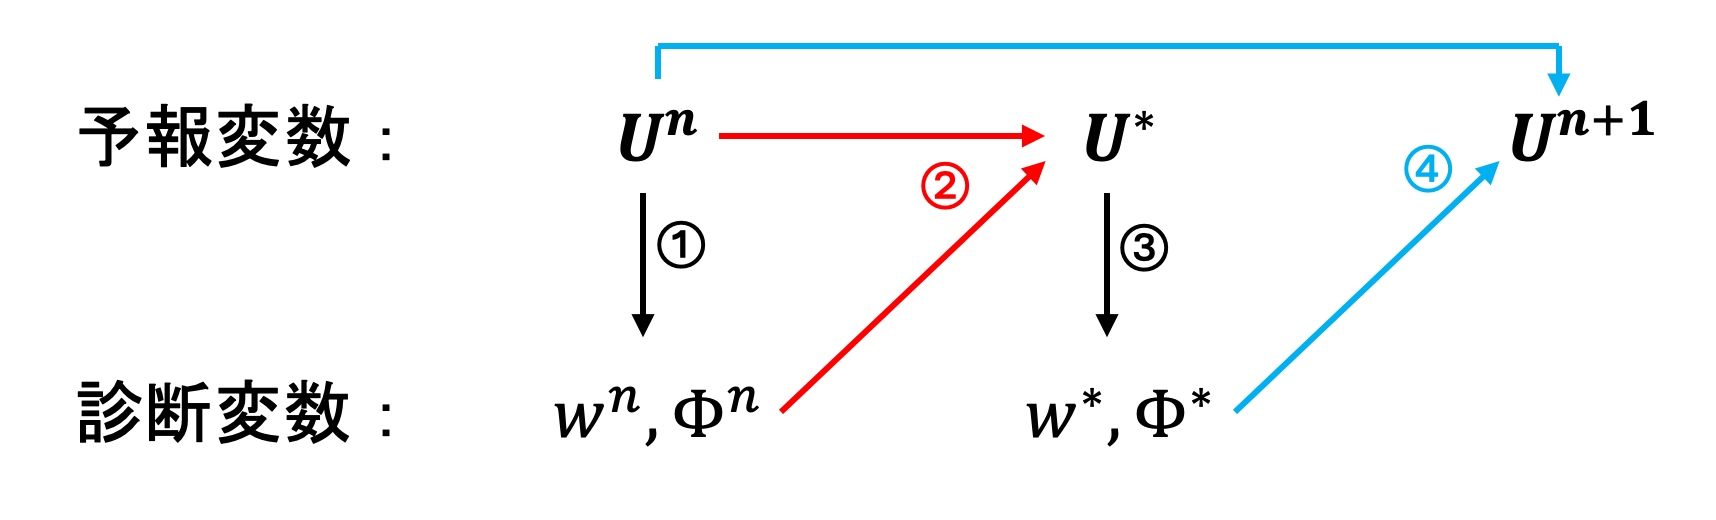
\includegraphics[width=0.5\textwidth]{./teximage/matsuno.png}
  \caption{松野スキームにおける計算の流れ。}
  \label{fig:1}
\end{figure}

\vs{0}
　ただし$\Phi$については$\partial \Phi/\partial\theta$を計算すれば十分である。まず$w$については、地表での境界条件より$w\bracketnormal{z=0,\theta}=0$であるから、$w\bracketnormal{z,\theta} = 0 + \int_{z=0}^z \partial w/\partial z' dz'$として計算すれば良い。すなわち
\neqns{l}{
  w^n\bracketnormal{z,\theta} = 0 + \dint_{0}^z \curlybracket{-\dfrac{1}{a\cos\theta}\pdifop{\theta}\bracketnormal{v^n\cos\theta}}dz'\\[5pt]
  w^*\bracketnormal{z,\theta} = 0 + \dint_{0}^z \underbrace{\curlybracket{-\dfrac{1}{a\cos\theta}\pdifop{\theta}\bracketnormal{v^*\cos\theta}}}_\text{以降$D[v^*]$のように書く。} dz'
}

として計算すれば良い。よって次に、もう一方の境界条件$w\bracketnormal{H,\theta}=0$が満たされるように$\partial\Phi/\partial \theta$を決定することを考える。今、
\neqn{
  w\bracketnormal{H,\theta} = \dint_0^H D[v]dz' = 0
}

が満たしたい境界条件である。この時、$n$ステップにおいて$w^n(H,\theta)=0$が満たされている状況で$n+1$ステップにおいても$w^{n+1}(H,\theta)=0$を満たすという条件を考えると、
\neqns{lcl}{
  \underbrace{\dint_0^H D[v^{n+1}]dz'}_{=w^{n+1}(H,\theta)} & \neqnsequal &\dint_0^H D\bigg[v^{n} + \Delta t \bigg\{-\dfrac{1}{a\cos\theta}\pdifop{\theta}\bracketnormal{v^{*2}\cos\theta}-\pdifop{z}\bracketnormal{w^*v^*}-fu^*\\
  && \qquad\qquad\qquad\qquad\qquad\qquad\qquad -\dfrac{u^{*2}\tan\theta}{a} + \pdifop{z}\bracketnormal{\nu\pdif{v^*}{z}}-\dfrac{1}{a}\pdif{\Phi^*}{\theta} \bigg\}\bigg]dz' \\[5pt]
  &\neqnsequal & \dint_0^H D\bigg[v^{n} + \Delta t \bigg\{R\left[u^* , v^* , w^*\right] -\dfrac{1}{a}\pdif{\Phi^*}{\theta}\bigg\}\bigg]dz'\\[5pt]
  &\neqnsequal & \underbrace{\dint_0^H D[v^{n}]dz'}_{=w^n(H,\theta)=0} + \Delta t \dint_0^H D\left[R\left[u^* , v^* , w^*\right] -\dfrac{1}{a}\pdif{\Phi^*}{\theta}\right]dz'\\[5pt]
  &\neqnsequal & 0
}

が満たされなければならない。\footnote{
  ただし途中で$v$方程式の圧力勾配項を除いた右辺$R$を以下のように定義している。\neqn{
    R\left[u^* , v^* , w^*\right]=-\dfrac{1}{a\cos\theta}\pdifop{\theta}\bracketnormal{v^{*2}\cos\theta}-\pdifop{z}\bracketnormal{w^*v^*}-fu^*-\dfrac{u^{*2}\tan\theta}{a} + \pdifop{z}\bracketnormal{\nu\pdif{v^*}{z}}
  }
}よって微分演算子$D$が$\int dz'$の外に出せることを踏まえれば、$\partial \Phi/\partial \theta$の計算に使うべき式は以下のようになる。\footnote{
  正確には、$D$を積分の外に出すことで$D[\int * dz']=0$という条件が現れ、ここから$\int * dz' = \frac{\text{const.}}{\cos\theta}$という条件が出るが、極で発散しないという条件を考えると定数は$0$出なければならず、結局$\int * dz' = 0$が導かれる。よって\refeqn{22}に帰着する。
}

\neqn{
  \dint_0^H \pdif{\Phi^*}{\theta}dz' = a\dint_0^H R\left[u^*,v^*,w^*\right]dz'\labeqn{22}
}

　ここで、静水圧平衡を用いれば$\Phi\bracketnormal{z,\theta} = \Phi\bracketnormal{0,\theta} + \int_0^z g\hat{\Theta}dz' = \Phi_\text{surface} + \int_0^z g\hat{\Theta}dz'$と計算できるので、次が成立する。

\neqn{
  \pdif{\Phi^*}{\theta} =\dif{\Phi^*_\text{surface}}{\theta}+ \int_0^z g\pdif{\hat{\Theta}^*}{\theta}dz'\labeqn{23}
}

よってこれを\refeqn{22}式に代入して整理すると

\neqn{
  \dif{\Phi^*_\text{surface}}{\theta} = \dfrac{a}{H}\dint_0^H R\left[u^*,v^*,w^*\right]dz'-\dfrac{1}{H}\dint_0^H\dint_0^z g \pdif{\hat{\Theta}^*}{\theta}dz'dz''
}

を得るので、\refeqn{23}に代入すれば最終的に$\partial \Phi/\partial \theta$が次のように求まることがわかる。

\neqn{
  \pdif{\Phi^*}{\theta} =\dfrac{a}{H}\dint_0^H R\left[u^*,v^*,w^*\right]dz' + \bracketnormal{\dint_0^z g\pdif{\hat{\Theta}^*}{\theta}dz' - \overline{\dint_0^z g\pdif{\hat{\Theta}^*}{\theta}dz'}}
}

ただし$\overline{\int_0^z g\frac{\partial{\hat{\Theta}}}{\partial{\theta}}dz'} = \frac{1}{H}\int_0^H \bracketnormal{\int_0^z g\frac{\partial{\hat{\Theta}}}{\partial{\theta}}dz'}dz''$である。よって$\Phi^*$の更新も同様に行うことにすれば、診断変数の計算式は明示的には次のようになる。
\neqns{lcl}{
  \pdif{\Phi^n}{\theta} &\neqnsequal& \dfrac{a}{H}\dint_0^H\curlybracket{-\dfrac{1}{a\cos\theta}\pdifop{\theta}\bracketnormal{v^{n2}\cos\theta}-\pdifop{z}\bracketnormal{w^nv^n}-fu^n-\dfrac{u^{n2}\tan\theta}{a} + \pdifop{z}\bracketnormal{\nu\pdif{v^n}{z}}}dz'\nonumber\\
  && \qquad\qquad\qquad\qquad\qquad + \dint_0^z g\pdif{\hat{\Theta}^n}{\theta}dz' -\dfrac{1}{H}\dint_0^H\bracketnormal{\dint_0^z g\pdif{\hat{\Theta}^n}{\theta}dz'}dz''\\[10pt]
  \pdif{\Phi^*}{\theta} &\neqnsequal& \dfrac{a}{H}\dint_0^H\curlybracket{-\dfrac{1}{a\cos\theta}\pdifop{\theta}\bracketnormal{v^{*2}\cos\theta}-\pdifop{z}\bracketnormal{w^*v^*}-fu^*-\dfrac{u^{*2}\tan\theta}{a} + \pdifop{z}\bracketnormal{\nu\pdif{v^*}{z}}}dz'\nonumber\\
  && \qquad\qquad\qquad\qquad\qquad  + \dint_0^z g\pdif{\hat{\Theta}^*}{\theta}dz' -\dfrac{1}{H}\dint_0^H\bracketnormal{\dint_0^z g\pdif{\hat{\Theta}^*}{\theta}dz'}dz''
}


\subsection{空間方向の離散化スキーム}
　今、子午面$\bracketnormal{\theta, z}\in [-\frac{\pi}{2},\frac{\pi}{2}]\times[0,H]$を$\theta$方向に$j=0\sim j_\text{max}-1$個、$z$方向に$k=0\sim k_\text{max}-1$個のセルに分割することを考える。（\reffig{2}左図参照。）この時、第$jk$番目のセルの中心に$u,\Theta$の$jk$番目の値を、セルの左辺中点に$v$の$jk$番目の値を、セルの下辺中点に$w,\Phi$の$jk$番目の値を配置する\footnote{
  すなわち流速に関してはちょうどセル境界を横切るような位置で取ることにする。
}。（\reffig{2}右図参照。）また、$\theta,z$についてはセル中心での値を$\theta_{j},z_{k}$と取ることにする。

\begin{figure}[!htbp]
    \centering
    \begin{subfigure}{0.58\textwidth}
        \centering
        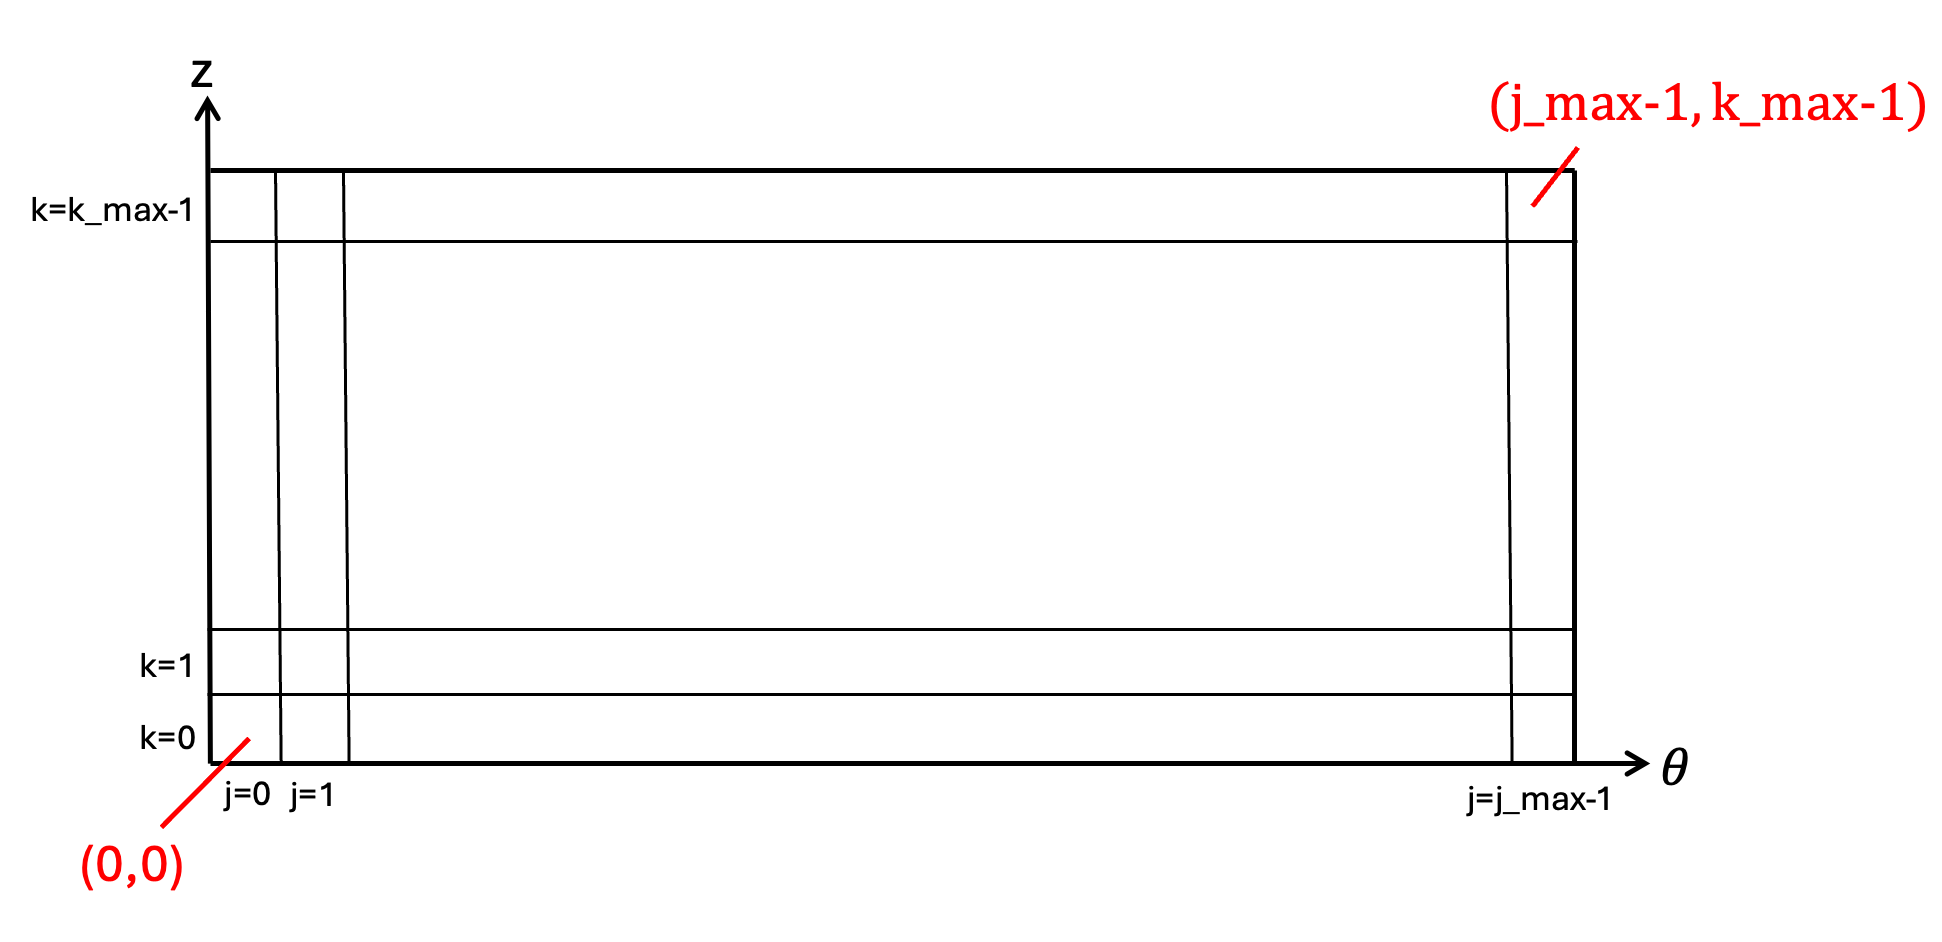
\includegraphics[width = \linewidth]{./teximage/grid.png}
    \end{subfigure}
    \begin{subfigure}{0.4\textwidth}
        \centering
        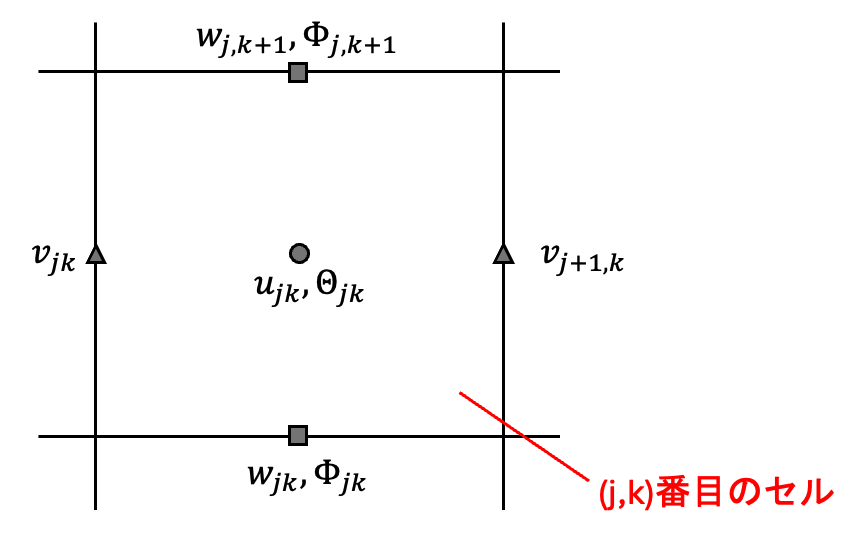
\includegraphics[width=\linewidth]{./teximage/grid2.png}
    \end{subfigure}
    \caption{空間のメッシュの切り方（左）と変数の配置（右）。}
    \label{fig:2}
\end{figure}

\vs{0}
　よって確保するメモリは次のようになる。（ただし$\Phi$について実際に保持するのは$\frac{\partial\Phi}{\partial\theta}$であることに注意。また、$\Theta_E$についてもメモリを確保する必要があることに注意。）
\neqns{ll}{
  \text{$u,\Theta,\Theta_E$について：}\quad &[0:j_\text{max}-1,0:k_\text{max}-1]\\
  \text{$w,\frac{\partial\Phi}{\partial\theta}$について：}\quad &[0:j_\text{max}-1,0:k_\text{max}]\\
  \text{$v$について：}\quad &[0:j_\text{max},0:k_\text{max}-1]\\
  \text{$\theta$について：}\quad &[0:j_\text{max}-1]\\
  \text{$z$について：}\quad &[0:k_\text{max}-1]
}

　ただし、実際には計算のために余分にメモリを確保しておく。また、変数が定義されていない点での値は平均操作により求めることにする。すなわち、たとえばセル中心での$v$の値は$v=\bracketnormal{v_{jk}+v_{j+1,k}}/2$のように計算する。



\FloatBarrier
\section{計算の実装}
　微分演算子は基本的に中央差分で評価することにする。また積分は、セル中心での値に$\Delta z$をかけて足し合わせることで評価する。その上で、$w,\Phi$の計算式、および$u,v,\Theta$の更新式の離散化を行う。

\subsection{\texorpdfstring{$w$の計算}{wの計算}}

　今、$w$は次のように計算されるのであった。
\neqn{
  w\bracketnormal{z,\theta} = 0 + \dint_{0}^z \curlybracket{-\dfrac{1}{a\cos\theta}\pdifop{\theta}\bracketnormal{v\cos\theta}}dz'
}

よって今$w_{jk}$がセル下辺に配置されていることに注意してこれを計算すると次のようになる。

\neqn{
  w_{jk} = \dsum_{k'=0}^{k-1}\left[\Delta z \curlybracket{-\dfrac{1}{a\cos\theta_j}\dfrac{v_{j+1,k'}\cos\bracketnormal{\dfrac{\theta_{j+1}+\theta_{j}}{2}}-v_{j,k'}\cos\bracketnormal{\dfrac{\theta_{j}+\theta_{j-1}}{2}}}{\Delta \theta}}\right]
}

よって、$w$を計算するルーチンを次のように定義すれば良い。
\vs{0.5}

\begin{algorithm}[!htbp]
  \caption*{\textbf{subroutine:} calculate\_w}
  \begin{algorithmic}[1]
    \Require $\theta[-2:j_\text{max}+1]$、$v[-1:j_\text{max}+1,0:k_\text{max}-1]$
    \Ensure $w[-1:j_\text{max},0:k_\text{max}]$
    \Statex
    \Do{$j=1,j_\text{max}$}
    \State $w=0$
    \Do{$k=0,k_\text{max}$}
    \State $w_{jk} = w$
    \State if $k=k_\text{max}$: cycle
    \State $w = w + \Delta z\bracketnormal{-\dfrac{1}{a\cos\theta_j}\dfrac{v_{j+1,k}\cos\bracketnormal{\dfrac{\theta_{j+1}+\theta_{j}}{2}}-v_{j,k}\cos\bracketnormal{\dfrac{\theta_{j}+\theta_{j-1}}{2}}}{\Delta \theta}}$
    \EndDo
    \EndDo
  \end{algorithmic}
\end{algorithm}

\subsection{\texorpdfstring{$\pdif{\Phi}{\theta}$の計算}{Phiの計算}}

　$\frac{\partial\Phi}{\partial\theta}$は次のように計算されるのであった。
\neqns{lcl}{
  \pdif{\Phi}{\theta} &\neqnsequal& \dfrac{a}{H}\dint_0^H\curlybracket{-\dfrac{1}{a\cos\theta}\pdifop{\theta}\bracketnormal{v^{2}\cos\theta}-\pdifop{z}\bracketnormal{wv}-fu-\dfrac{u^{2}\tan\theta}{a} + \pdifop{z}\bracketnormal{\nu\pdif{v}{z}}}dz'\nonumber\\
  && \qquad\qquad\qquad\qquad\qquad + \dint_0^z g\pdif{\hat{\Theta}}{\theta}dz' -\dfrac{1}{H}\dint_0^H\bracketnormal{\dint_0^z g\pdif{\hat{\Theta}}{\theta}dz'}dz''\labeqn{35}
}

よってあらかじめ$\int _0^z g\frac{\partial\hat{\Theta}}{\partial\theta}dz'$をセル下辺で評価しておくと見通しが良い。今積分はセル中心での値に厚み$\Delta z$をかけて足し合わせることで評価することにしているので、これは次のように計算することができる。

\neqn{
  \bracketnormal{\dint _0^z g\frac{\partial\hat{\Theta}}{\partial\theta}dz'}_{jk} = \dsum_{k'=0}^{k-1}\bracketnormal{\Delta z g\dfrac{\hat{\Theta}_{j+1,k'}-\hat{\Theta}_{j-1,k'}}{2\Delta \theta}}
}

また\refeqn{35}の第一項の積分は次のように計算することができる。

\neqns{l}{
  \dint_0^H\curlybracket{-\dfrac{1}{a\cos\theta}\pdifop{\theta}\bracketnormal{v^{2}\cos\theta}-\pdifop{z}\bracketnormal{wv}-fu-\dfrac{u^{2}\tan\theta}{a} + \pdifop{z}\bracketnormal{\nu\pdif{v}{z}}}dz'\nonumber \\[5pt]
  \qquad = \dsum_{k=0}^{k_\text{max}-1} \Bigg[\Delta z\Bigg\{-\dfrac{1}{a\cos\theta_j}\dfrac{v_{j+1,k}^2 \cos\dfrac{\theta_j + \theta_{j+1}}{2}-v_{j,k}^2 \cos\dfrac{\theta_{j-1} + \theta_{j}}{2}}{\Delta \theta}\nonumber \\[5pt]
  \qquad\qquad - \dfrac{w_{j,k+1}\dfrac{v_{jk}+v_{j+1,k}+v_{j,k+1}+v_{j+1,k+1}}{4}-w_{j,k}\dfrac{v_{j,k-1}+v_{j+1,k-1}+v_{j,k}+v_{j+1,k}}{4}}{\Delta z}\nonumber\\[5pt]
  \qquad\qquad -2\Omega \sin\theta_{j}u_{jk}-\dfrac{u_{jk}^2\tan\theta_j}{a}\nonumber\\[5pt]
  \qquad\qquad+ \dfrac{\nu}{\Delta z}\bracketnormal{\dfrac{\dfrac{v_{j,k+1}+v_{j+1,k+1}}{2}-\dfrac{v_{jk}+v_{j+1,k}}{2}}{\Delta z}-\dfrac{\dfrac{v_{jk}+v_{j+1,k}}{2}-\dfrac{v_{j,k-1}+v_{j+1,k-1}}{2}}{\Delta z}}
  \Bigg\}\Bigg]
}

よってこれらを用いて$\frac{\partial\Phi}{\partial\theta}$を計算するルーチンをcalculate\_partial\_Phiのように定めればいい。

\vs{0.5}

\begin{algorithm}[!htbp]
  \caption*{\textbf{subroutine:} calculate\_partial\_Phi}
  \begin{algorithmic}[1]
    \Require $\theta[-2:j_\text{max}+1]$、$u[-1:j_\text{max},0:k_\text{max}-1]$、$v[-1:j_\text{max}+1,-1:k_\text{max}]$、$\hat{\Theta}[-2,j_\text{max}+1,0:k_\text{max}-1]$、$w[-1:j_\text{max},0:k_\text{max}]$
    \Ensure $\pdif{\Phi}{\theta}[-1:j_\text{max},0:k_\text{max}]$
    \Statex
    \Do{$j=-1,j_\text{max}$}
    \State \Comment{温位の積分をセル下辺で評価する}
    \State $\text{integral} = 0$
    \Do{$k=0,k_\text{max}$}
    \State $\bracketnormal{\dint_0^z g\pdif{\hat{\Theta}}{\theta}dz'}_{jk} = \text{integral} $
    \State if $k=k_\text{max}$: cycle
    \State $\text{integral}=\text{integral} + \Delta z g\dfrac{\hat{\Theta}_{j+1,k}-\hat{\Theta}_{j-1,k}}{2\Delta \theta}$
    \EndDo
    \State \Comment{第三項の積分の評価}
    \State $\text{term3}=0$
    \Do{$k=0,k_\text{max}-1$}
    \State $\text{term3} = \text{term3} + \Delta z\dfrac{\bracketnormal{\dint_0^z g\pdif{\hat{\Theta}}{\theta}dz'}_{jk} + \bracketnormal{\dint_0^z g\pdif{\hat{\Theta}}{\theta}dz'}_{jk+1} }{2}$
    \EndDo
    \State $\text{term3} = \text{term3}\times\bracketnormal{-\dfrac{1}{H}}$
    \State \Comment{第一項の積分の評価}
    \State $\text{term1}=0$
    \Do{$k=0,k_\text{max}-1$}
    \State $\begin{aligned}[t]
    &\text{term1} = \text{term1} + \Bigg[\Delta z\Bigg\{-\dfrac{1}{a\cos\theta_j}\dfrac{v_{j+1,k}^2 \cos\dfrac{\theta_j + \theta_{j+1}}{2}-v_{j,k}^2 \cos\dfrac{\theta_{j-1} + \theta_{j}}{2}}{\Delta \theta} \\[5pt]
    &\qquad\qquad - \dfrac{w_{j,k+1}\dfrac{v_{jk}+v_{j+1,k}+v_{j,k+1}+v_{j+1,k+1}}{4}-w_{j,k}\dfrac{v_{j,k-1}+v_{j+1,k-1}+v_{j,k}+v_{j+1,k}}{4}}{\Delta z}\\[5pt]
    &\qquad\qquad -2\Omega \sin\theta_{j}u_{jk}-\dfrac{u_{jk}^2\tan\theta_j}{a}\\[5pt]
    &\qquad\qquad+ \dfrac{\nu}{\Delta z}\bracketnormal{\dfrac{\dfrac{v_{j,k+1}+v_{j+1,k+1}}{2}-\dfrac{v_{jk}+v_{j+1,k}}{2}}{\Delta z}-\dfrac{\dfrac{v_{jk}+v_{j+1,k}}{2}-\dfrac{v_{j,k-1}+v_{j+1,k-1}}{2}}{\Delta z}}\Bigg\}\Bigg]
    \end{aligned}$
    \EndDo
    \State $\text{term1} = \text{term1}\times\dfrac{a}{H}$
    \State \Comment{最終的に求めたいPhiの偏微分の下辺での評価}
    \Do{$k=0,k_\text{max}$}
    \State $\bracketnormal{\pdif{\Phi}{\theta}}_{jk} = \text{term1}+\text{term3} + \bracketnormal{\dint_0^z g\pdif{\hat{\Theta}}{\theta}dz'}_{jk}$
    \EndDo
    \EndDo
  \end{algorithmic}
\end{algorithm}

\subsection{\texorpdfstring{$u$の更新}{uの計算}}

　$u$の更新式は次のようになる。

\neqn{
  u^\text{out} = u^n + \Delta t\bracketnormal{-\dfrac{1}{a\cos\theta}\pdifop{\theta}\bracketnormal{vu\cos\theta}-\pdifop{z}\bracketnormal{wu}+fv+\dfrac{uv\tan\theta }{a}+\pdifop{z}\bracketnormal{\nu \pdif{u}{z}}}
}

ただし$u^\text{out} = u^{n+1}\;\text{or}\;u^*$であり、右辺の$u,v,w$には$u^n,v^n,w^n$ないし$u^*,v^*,w^*$が入る。その上で、上式をセル中心で評価すると次のようになる。

\neqns{l}{
  u_{jk}^\text{out} = u^n_{jk} + \Delta t\Bigg\{-\dfrac{1}{a\cos\theta_j}\dfrac{\dfrac{u_{jk}+u_{j+1,k}}{2}v_{j+1,k}\cos\dfrac{\theta_{j+1}+\theta_{j}}{2}-\dfrac{u_{j-1,k}+u_{j,k}}{2}v_{j,k}\cos\dfrac{\theta_{j}+\theta_{j-1}}{2}}{\Delta \theta} \\[5pt]
  \qquad\qquad - \dfrac{\dfrac{u_{jk}+u_{j,k+1}}{2}w_{j,k+1}-\dfrac{u_{j,k-1}+u_{j,k}}{2}w_{j,k}}{\Delta z} + 2\Omega\sin\theta_j\dfrac{v_{jk}+v_{j+1,k}}{2}\Bigg\}
}

\subsection{境界の外側のセルの更新}

\end{document}


